\section{PHƯƠNG TRÌNH ĐƯỜNG THẲNG}
%\subsection{Tóm tắt lí thuyết}
%\subsubsection{Phương trình tổng quát của đường thẳng}
%\begin{dn}
%	Véc-tơ $\vec{n}$ khác $\vec{0}$ được gọi là véc-tơ pháp tuyến của đường thẳng $\Delta$ nếu giá của nó vuông góc với $\Delta$.
%\end{dn}
%\begin{nx}\hfill
%	\begin{itemize}
%		\item Nếu $\vec{n}$ là véc-tơ pháp tuyến của đường thẳng $\Delta$ thì $k\vec{n}$ ($k \ne 0$) cũng là véc-tơ pháp tuyến của $\Delta$.
%		\item Đường thẳng hoàn toàn xác định nếu biết một điểm và một véc-tơ pháp tuyến của nó.
%	\end{itemize}
%\end{nx}
%
%\begin{vd}
%	Trong mặt phẳng tọa độ, cho tam giác có ba đỉnh là $A(3;1)$, $B(4;0)$, $C(5;3)$. Hãy chỉ ra  một véc-tơ pháp tuyến của đường trung trực của đoạn thẳng $AB$ và một véc-tơ pháp tuyến của đường cao kẻ từ $A$ của tam giác $ABC$.
%	\loigiai{
%		Đường trung trực của đoạn $AB$ vuông góc với $AB$ nên có một véc-tơ pháp tuyến là $\vec{AB}(1;-1)$.
%		Đường cao kẻ từ kẻ từ $A$ của tam giác $ABC$ vuông góc với $BC$ nên có một  véc-tơ pháp tuyến là $\vec{BC}(1;3)$.
%	}
%\end{vd}
%
%\begin{nx}
%	Trong mặt phẳng tọa độ, mọi đường thẳng đều có phương trình tổng quát dạng $ax+by+c=0$, với $a$ và  $b$ không đồng thời bằng $0$. Ngược lại, mỗi phương trình dạng $ax+by+c=0$,  với $a$ và  $b$ không đồng thời bằng $0$, đều là phương trình của một đường thẳng, nhận $\vec{n}(a;b)$ là một véc-tơ pháp tuyến.
%\end{nx}
%\begin{vd}
%	Trong mặt phẳng tọa độ, lập phương trình tổng quát của đường thẳng $\Delta$ đi qua điểm $A(2;1)$ và nhận $\vec{n}(3;4)$ là một véc-tơ pháp tuyến.
%	\loigiai{
%		Đường thẳng $\Delta$ có phương trình là $3(x-2)+4(y-1)=0$ hay $3x+4y-10=0$.
%	}
%\end{vd}
%
%\begin{vd}
%	Trong mặt phẳng tọa độ, cho tam giác có ba đỉnh $A(-1;5)$, $B(2;3)$, $C(6;1)$. Lập phương trình tổng quát của đường cao kẻ từ $A$ của tam giác $ABC$.
%	\loigiai{Ta có $\vec{BC}(4;-2)$.\\
%		Đường cao kẻ từ kẻ từ $A$ của tam giác $ABC$ vuông góc với $BC$ nên có một  véc-tơ pháp tuyến là $\vec{n}(2;-1)$.\\
%		Đường thẳng $\Delta$ có phương trình là $2(x+1)-(y-5)=0$ hay $2x-y+7=0$.
%	}
%\end{vd}
%
%\begin{vd}
%	Trong mặt phẳng tọa độ, lập phương trình tổng quát của đường thẳng $\Delta$ đi qua điểm $A(0;b)$ và có véc-tơ pháp tuyến  $\vec{n}(a;-1)$ với $a$, $b$ là các số cho trước. Hãy chỉ ra mối liên hệ giữa đường thẳng $\Delta$ với đồ thị của hàm số $y=ax+b$.
%	\loigiai{
%		Đường thẳng $\Delta$ có phương trình là $a(x-0)-1(y-b)=0$ hay $ax-y+b=0$.\\
%		Đường thẳng $\Delta$ là tập hợp những điểm $M(x;y)$ thoả mãn $ax-y+b=0$, hay là $y=ax+b$.\\
%		Do đó, đường thẳng $\Delta: ax-y+b=0$ chính là đồ thị hàm số $y=ax+b$.
%	}
%\end{vd}
%
%\begin{vd}
%	Hãy chỉ ra một véc-tơ pháp tuyến của đường thẳng $\Delta \colon y=3x+4$.
%	\loigiai{
%		Đường thẳng $\Delta$ có một véc-tơ pháp tuyến là $\vec{n}(3;-1)$.
%	}
%\end{vd}
%\begin{nx}
%	Trong mặt phẳng tọa độ, cho đường thẳng $ \Delta \colon ax+by+c=0$.
%	\begin{itemize}
%		\item Nếu $b=0$ thì phương trình có thể đưa về dạng $x=m$ (với $m=-\dfrac{c}{a}$) và $\Delta$ vuông góc với $Ox$.
%		\item Nếu $b \ne 0$ thì phương trình có thể đưa về dạng $y=nx+p$ (với $n=-\dfrac{a}{b}$, $m=-\dfrac{c}{b}$).
%	\end{itemize}
%\end{nx}
%
%\subsubsection{Phương trình tham số của đường thẳng}
%\begin{dn}
%	Véc-tơ $\vec{u}$ khác $\vec{0}$ được gọi là véc-tơ chỉ phương  của đường thẳng $\Delta$ nếu giá của nó song song hoặc trùng  với $\Delta$.
%\end{dn}
%\begin{nx}
%	\begin{itemize}
%		\item Nếu $\vec{u}$ là véc-tơ chỉ phương  của đường thẳng $\Delta$ thì $k\vec{u}$ ($k \ne 0$) cũng là véc-tơ chỉ phương của $\Delta$.
%		\item Đường thẳng hoàn toàn xác định nếu biết một điểm và một véc-tơ chỉ phương của nó.
%		\item Véc-tơ $\vec{n}(a;b)$ vuông góc với các véc-tơ $\vec{u}(-b;a)$ và $\vec{v}(b;-a)$ nên nếu $\vec{n}$ là véc-tơ pháp tuyến của đường thẳng $\Delta$ thì $\vec{u}$, $\vec{v}$ là hai véc-tơ chỉ phương của đường thẳng đó và ngược lại.
%	\end{itemize}
%\end{nx}
%
%\begin{vd}
%	Trong mặt phẳng tọa độ, cho  $A(3;2)$, $B(1;-4)$. Hãy chỉ ra  hai  véc-tơ chỉ phương  của đường  thẳng $AB$.
%	\loigiai{
%		Đường  thẳng $AB$ nhận  $\vec{AB}(-2;-6)$ là một véc-tơ chỉ phương.\\
%		Lấy  $\vec{u}=-\dfrac{1}{2}\vec{AB}=(1;3)$, khi đó  $\vec{u}$ cũng là một véc-tơ chỉ phương của đường thẳng $AB$.
%	}
%\end{vd}
%
%\begin{vd}
%	Hãy chỉ ra một véc-tơ  chỉ phương  của đường thẳng $\Delta \colon 2x-y+1=0$.
%	\loigiai{
%		Đường thẳng $\Delta$ có một véc-tơ chỉ phương là $\vec{n}(1;2)$.
%	}
%\end{vd}
%\begin{dn}
%	Cho đường thẳng $\Delta$ đi qua điểm $A(x_0;y_0)$ và có véc-tơ chỉ phươn g$\vec{u}(a;b)$. Khi đó điểm $M(x;y)$  thuộc  đường thẳng $\Delta$ khi và chỉ khi tôn tại số thực $t$ sao cho $\vec{AM}=t\vec{u}$, hay 
%	\[\heva{&x=x_0+at\\&y=y_0+bt.} \quad \quad (2)\]
%	Hệ $(2)$ được gọi là phương trình tham số của đường thẳng $\Delta$ ($t$ là tham số).
%\end{dn}
%
%\begin{vd}
%	Lập phương trình tham số của đường thẳng $\Delta$ đi qua $M(2;-3)$ và có  véc-tơ  chỉ phương $\vec{u}(4;-1)$.
%	\loigiai{
%		Phương trình tham số của đường thẳng $\Delta$  là $\heva{&x=2+4t\\&y=-3-t.}$
%	}
%\end{vd}
%
%\begin{vd}
%	Lập phương trình tham số của đường thẳng $\Delta$ đi qua $M(-1;2)$ và song song với đường thẳng $d \colon 3x-4y-1=0$.
%	\loigiai{ Đường thẳng $\Delta$  song song với đường thẳng $d \colon 3x-4y-1=0$ nên có một véc-tơ chỉ phương là  $\vec{u}(4;3)$.\\
%		Phương trình tham số của đường thẳng $\Delta$  là $\heva{&x=-1+4t\\&y=2+3t.}$
%	}
%\end{vd}
%
%\begin{vd}
%	Lập phương trình tham số của đường thẳng $\Delta$ đi qua hai điểm  $A(2;3)$ và $B(1;5)$.
%	\loigiai{ Đường thẳng $\Delta$  đi qua hai điểm  $A(2;3)$ và $B(1;5)$  nên có một véc-tơ chỉ phương là  $\vec{u}=\vec{AB}=(-1;2)$.\\
%		Phương trình tham số của đường thẳng $\Delta$  là $\heva{&x=2-t\\&y=3+2t.}$
%	}
%\end{vd}
%
%\begin{vd}
%	Lập phương trình tham số và phương trình tổng quát của đường thẳng $\Delta$ đi qua hai điểm  phân biệt  $A(x_1;y_1)$ và $B(x_2;y_2)$ cho trước.
%	\loigiai{ Đường thẳng $\Delta$  đi qua hai điểm $A(x_1;y_1)$ và $B(x_2;y_2)$  nên có một véc-tơ chỉ phương là  $\vec{u}=\vec{AB}=(x_2-x_1;y_2-y_1)$.\\
%		Phương trình tham số của đường thẳng $\Delta$  là $\heva{&x=x_1+(x_2-x_1)t\\&y=y_1+(x_2-x_1)t.}$\\
%		Ta có một véc-tơ pháp tuyến của đường thẳng $\Delta$ là $\vec{n}=(y_1-y_2;x_2-x_1)$.\\ Phương trình tổng quát của $\Delta$ là $((y_1-y_2)(x-x_1)+(x_2-x_1)(y-y_1)=0$
%	}
%\end{vd}

\subsection{Các dạng toán thường gặp}
\begin{dang}{Bài toán tìm điểm trên parabol}
	Cho parabol có phương trình chính tắc $y^2=2 p x, p>0$. Khi đó:
	\begin{itemize}
		\item Parabol có tiêu điểm $F\left(\dfrac{p}{2} ; 0\right)$ và đường chuẩn $\Delta: x=-\dfrac{p}{2}$;
		\item Với điểm $M(x ; y)$ thuộc parabol, đoạn thẳng $M F$ được gọi là bán kính qua tiêu củ $M$ và có độ dài $M F=x+\dfrac{p}{2}$.
		\item Với mọi điểm $M(x ; y)$ thuộc parabol, tỉ số $\dfrac{M F}{\mathrm{d}(M, \Delta)}$ luôn bằng $ 1  $. Ta nói parabol có tâm sai bằng $ 1 $.
	\end{itemize}
	
\end{dang}
\begin{vd}
	Cho parabol có phương trình $ y^2=4x $.
	\begin{enumerate}
		\item Tìm tọa độ tiêu điểm và phương trình đường chuẩn của parabol.
		\item Tính bán kính qua tiêu của điểm $M$ thuộc parabol và có hoành độ bằng $ 3 $.
	\end{enumerate}
\loigiai{
	\begin{enumerate}
		\item Từ phương trình chính tắc của parabol, ta có $ 2p=4 \Leftrightarrow p=2 $.\\
		Vậy parabol có tiêu điểm là $F(1 ; 0)$ và đường chuẩn là $x=-1$.
		\item Theo công thức bán kính qua tiêu ta có $M F=3+1=4$.
	\end{enumerate}
	
}
	
	\end{vd}
\begin{vd}
	 Cho parabol có phương trình $y^2=8 x$. Tìm tọa độ tiêu điểm và phương trình đường chuẩn của parabol. Tính bán kính qua tiêu của điểm $M$ thuộc parabol biết điểm $M$ có tung độ bằng $4 .$
	 \loigiai{
	 	Từ phương trình chính tắc của parabol, ta có $ 2p=8 \Leftrightarrow p=4 $.\\
	 	Tọa độ tiêu điểm của parabol là $F=\left(2;0\right)   $.\\
	 	Phương trình đường chuẩn của parabol là $ x=2 $.\\
	 	Bán kính qua tiêu của điểm $M$ thuộc parabol biết điểm $M$ có tung độ bằng $4  $ là $ MF=3+2=6 $.
	 	
	 }
	\end{vd}
\begin{vd}
	  Cho parabol $y^2=6 x$.
	  \begin{enumerate}
	  	\item Tìm tọa độ tiêu điểm và phương trình đường chuẩn của parabol.
	  	\item  Giả sử $M$ là điểm thuộc parabol có hoành độ là $4 .$ Tính bán kính qua tiêu của điểm $M$.
	  \end{enumerate}
\loigiai{
	\begin{enumerate}
		\item  Ta có  $2 p=6$, suy ra $p=3$.\\
		Tiêu điểm của parabol là $F\left(\dfrac{3}{2} ; 0\right)$.\\
		Đường chuẩn của parabol có phương trình là $x=-\dfrac{3}{2}$.
		\item  Bán kính qua tiêu của điểm $M$ là $M F=4+\dfrac{3}{2}=5,5$.
	\end{enumerate}
}
	
	\end{vd}
 
 \begin{vd}
 	Tính bán kính qua tiêu của điểm $M(1 ; 2)$ trên parabol $(P): y^2=4 x$.
 	\loigiai{
  Từ phương trình chính tắc của parabol, ta có $ 2p=4 \Leftrightarrow p=2 $.\\
 		Vậy parabol có tiêu điểm là $F(1 ; 0)$ và đường chuẩn là $x=-1$.\\
  Theo công thức bán kính qua tiêu ta có $M F=1+1=2$.
 
}
 	\end{vd}
 
 \begin{vd}
  Chứng minh rằng trong các điểm thuộc parabol thì đỉnh parabol có khoảng cách tới tiêu điểm nhỏ nhất và khoảng cách đó bằng một nửa tham số tiêu.
  \loigiai{
  Giả sử parabol có phương trình chính tắc là $y^2=2 p x, p>0$. Với điểm $M\left(x_0 ; y_0\right)$ bất kì thuộc parabol, ta có $x_0 \geq 0$. Do đó, theo công thức bán kính qua tiêu, ta có $M F=x_0+\dfrac{p}{2} \geq \dfrac{p}{2}$. Dấu đẳng thức xảy ra khi và chỉ khi $x_0=0$ (và do đó $y_0=0$), tức là $M$ trùng với đỉnh $O(0 ; 0)$ của parabol. Từ đó, ta nhận được điều phải chứng minh.
  	
  }
 	\end{vd}
 
 
 
 \begin{bt} 
 	\immini{
 		Viết phương trình của parabol $(P)$ có tiêu điểm $F(3;0)$.
 	}{
 		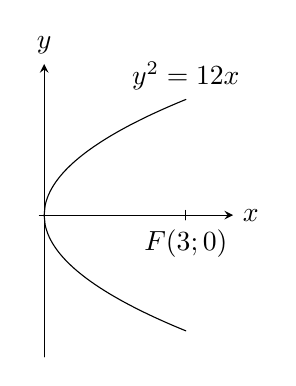
\begin{tikzpicture}[domain=0:3,line join = round, line cap = round,>=stealth,scale=0.6]
 			\draw[->] (-0.1,0) -- (4,0) node[right] {$x$};
 			\draw[->] (0,-3) -- (0,3.2) node[above] {$y$};
 			\draw[smooth, samples=150] plot (\x,{-(2*(\x))^(0.5)});
 			\draw[smooth, samples=150] plot (\x,{(2*(\x))^(0.5)}) node[above]{$y^2=12x$};
 			\draw (3,0.1)--(3,-0.1) node[below]{$F(3;0)$};
 		\end{tikzpicture}  
 	}
 	\loigiai{
 		Parabol $(P)$ có tiêu điểm $F(3;0)$ nên ta có: $\dfrac{p}{2}=3$, suy ra $p=6$. Vậy $(P)$ có phương trình $y^2=12x$.
 	}
 \end{bt}
\begin{bt} 
Tìm tọa độ tiêu điểm, phương trình đường chuẩn của các parabol sau
\begin{listEX}[3]
	\item $y^2=4x$;
	\item $y^2=2x$;
	\item $y^2=-6x$.
\end{listEX}
\loigiai{
	\begin{enumerate}
		\item Parabol $y^2=4x$ có $p=2$ nên tọa độ tiêu điểm là $F(1;0)$ và phương trình đường chuẩn là $x+1=0$.
		\item Parabol $y^2=2x$ có $p=1$ nên tọa độ tiêu điểm là $F\left(\dfrac{1}{2};0 \right) $ và phương trình đường chuẩn là $$x+\dfrac{1}{2}=0.$$
	\end{enumerate}	
}
\end{bt}
\begin{bt}%[Tex hóa SGK CD-CT,T7/22, Ninh Tiến Nam]%[0H3B5-2]
Viết phương trình chính tắc của parabol 	 thoả mãn các điều kiện
\begin{enumerate}
	\item Tiêu điểm $(8;0)$;
	\item Khoảng cách từ tiêu điểm đến đường chuẩn bằng $4$.
\end{enumerate}
\loigiai{\begin{enumerate}
		\item Theo giả thiết suy ra parabol có $\dfrac{p}{2}=8\Rightarrow p=16$.\\
		Vậy phương trình parabol là $y^2=32x$.
		\item Khoảng cách từ tiêu điểm đến đường chuẩn bằng $4$ nên $p=4$.\\
		Vậy phương trình parabol là $y^2=8x$.
	\end{enumerate}
}
\end{bt}

\begin{dang}{Bài toán thực tế}
\begin{itemize}
	\item Mô hình hóa bài toán
	\item Đưa bài toán về các kiến thức parabol
\end{itemize}
	
\end{dang}
\begin{vd}
	  Một sao chổi chuyển động theo quỹ đạo parabol nhận tâm Mặt Trời làm tiêu điểm. Khoảng cách ngắn nhất từ sao chổi đến tâm Mặt Trời là 106 km. Lập phương trình chính tắc của quỹ đạo theo đơn vị kilômét. Hỏi khi sao chổi nằm trên đường vuông góc với trục đối xứng của quỹ đạo tại tâm Mặt Trời, thì khoảng cách từ sao chổi đến tâm Mặt Trời là bao nhiêu kilômét?
	  \loigiai{
	  	\immini
	  	{
	  		Chọn hệ trục như hình vẽ với mặt trời trùng tiêu điểm $ F $.\\
	  		Khoảng cách từ mặt trời đến sao chổi ngắn nhất là $ 106 $ km nên điểm $ F=(106;0) $ và $ p=212 $.\\
	  		Do đó phương trình chính tắc của parabol là $ y^2 =424 x $.
	  	}
	  	{
	  		\begin{tikzpicture}[line join=round, line cap=round,>=stealth,scale=0.6]
	  			\tikzset{label style/.style={font=\footnotesize}}
	  			\draw[->] (-1.1,0)--(3.1,0) node[below left] {$x$};
	  			\draw[->] (0,-2.5)--(0,2.5) node[below left] {$y$};
	  			\draw (0,0) node [below left] {$O$};
	  			\begin{scope}
	  				\clip (-2,-4) rectangle (4,4);
	  				\draw[samples=200,domain=0:3,smooth,variable=\x] plot (\x,{sqrt((\x))});
	  				\draw[samples=200,domain=0:3,smooth,variable=\x] plot (\x,{-sqrt((\x))});
	  			\end{scope}
	  			\filldraw[black] (1,0) circle (1pt) node[below]{$ F $};
	  		\end{tikzpicture}
	  	}
	  }
	\end{vd}

\begin{vd} 
	\immini{Một chiếc đèn có mặt cắt ngang là hình parabol như hình bên. Hình parabol có chiều rộng giữa hai mép vành là $AB=40$cm và chiều sâu $h=30$cm ($h$ bằng khoảng cách từ $O$ đến $AB$). Bóng đèn nằm ở tiêu điểm $S$. Viết phương trình chính tắc của parabol đó.}
	{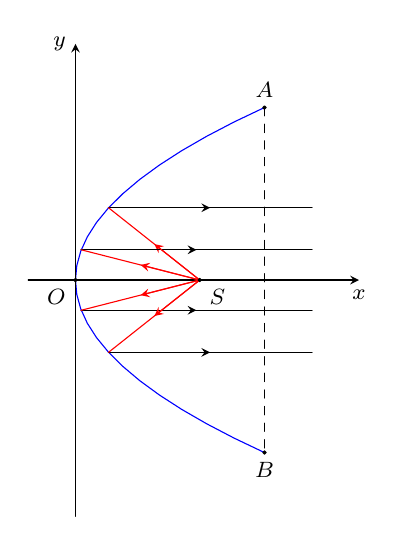
\begin{tikzpicture}[scale=0.6, font=\footnotesize, line join=round, line cap=round, >=stealth]
			
			\draw[domain=-3.65:3.65, blue,] plot({3/10*(\x)^2},\x);
			%\draw[gray!10] (-1,-1) grid (5,5);
			\draw[->] (-1,0)--(6,0) node[below]{$x$};
			\draw[->] (0,-5)--(0,5) node[left]{$y$};
			\coordinate (A) at (4,3.65); 
			\coordinate (B) at (4,-3.65); 
			\coordinate (O) at (0,0); 
			\coordinate (C) at (0.12,0.64); 
			\coordinate (C') at (0.12,-0.64); 
			\coordinate (D) at (0.7,1.53); 
			\coordinate (D') at (0.7,-1.53); 
			\coordinate (F) at (5.01,1.53); 
			\coordinate (F') at (5.01,-1.53); 
			\coordinate (G) at (5.01,0.64); 
			\coordinate (G') at (5.01,-0.64); 
			\coordinate (E) at (2.63,0); 
			\coordinate (H1) at (1.67,0.76); 
			\coordinate (H2) at (1.67,-0.76); 
			\coordinate (H3) at (1.38,0.32); 
			\coordinate (H4) at (1.38,-0.32); 
			\coordinate (K1) at (2.85,1.53); 
			\coordinate (K2) at (2.85,-1.53); 
			\coordinate (K3) at (2.56,0.64); 
			\coordinate (K4) at (2.56,-0.64); 
			\draw  (F)--(D) (G)--(C) (F')--(D') (G')--(C') ;
			\draw[dashed] (A)--(B);
			\draw[red,->] (E)--(H1); 
			\draw[->] (D)--(K1) ;
			\draw[red,->] (E)--(H3); 
			\draw[->] (C)--(K3) ;
			\draw[red,->] (E)--(H4); 
			\draw[->] (C')--(K4) ;
			\draw[red,->] (E)--(H2); 
			\draw[->] (D')--(K2) ;
			
			\draw[red] (E)--(C) (E)--(D) (E)--(C') (E)--(D');
			
			\draw[fill=black] (A) circle (1pt) node [above] {$A$};
			\draw[fill=black] (B) circle (1pt) node [below] {$B$};
			\draw[fill=black] (E) circle (1pt) node [below right] {$S$};
			\draw[fill=black] (O) circle (1pt) node [below left] {$O$};
	\end{tikzpicture}}
	
	\loigiai{Gắn hình parabol vào hệ trục như đề bài, dựa vào giả thiết bài toán ta có tọa độ điểm $A(30;20)$. Parabol đi qua điểm $A$ nên ta có phương trình 
		\begin{eqnarray*}
			20^2=2p\cdot 30 \Leftrightarrow p=\dfrac{20}{3}.
		\end{eqnarray*}
		Vậy ta có phương trình chính tắc của parabol đó là $y^2=\dfrac{40x}{3}$.	
	}
\end{vd}

\begin{vd} 
	\immini{
		Cổng của một ngôi trường có dạng một parabol. Để đo chiều cao $h$ của cổng, một người đo khoảng cách giữa hai chân cổng được $9$ m, người đó thấy nếu đứng cách chân cổng $0{,}5$ m thì đầu chạm cổng. Cho biết người này cao $1{,}6$ m, hãy tính chiều cao của cổng.
	}{
		\begin{tikzpicture}[scale=0.5, font=\footnotesize, line join=round, line cap=round, >=stealth]
			\tikzset{cua-phu/.pic={
					\def\xm{3};
					\def\xn{3.05};
					\pgfmathsetmacro\ym{-(496/1125)*(\xm)^2+6.2};
					\pgfmathsetmacro\yn{-(496/1125)*(\xn)^2+6.2};
					\path
					(0,0) coordinate (O)
					(\xm,\ym) coordinate (M)
					(\xn,\yn) coordinate (N)
					(3.75,0) coordinate (A)
					;
					%vẽ cửa bên phải
					\fill[color=yellow!90!gray] plot[smooth, samples=200, domain=\xn:3.75] (\x,{-(496/1125)*(\x)^2+6.2})--(3.75,\yn)coordinate(A')--(N)--cycle;
					\fill[color=yellow!80!gray](A')++(0,-0.4) coordinate (B)--++(1.5,0) coordinate(C)--(5.5,\yn) coordinate (E)--(A');
					\fill[color=yellow!80!gray](C)--++(0,-1.6)coordinate (D)--($(E)+(0,-2.1)$)coordinate (F)--(E)--(C);
					\fill[color=yellow!90!gray](F)--++(1,0) coordinate(G)--(6.5,\yn) coordinate(N')--(E)--(F);
					\fill[color=yellow!30]($(E)+(0.2,-0.2)$)coordinate(E')--($(F)+(0.2,0.2)$)coordinate(F')--($(G)+(-0.2,0.2)$)coordinate(G')--($(N')+(-0.2,-0.2)$)coordinate(N'')--cycle;
					\fill[color=yellow!30] (M)--(6.5,\ym) coordinate (M')--(N')--(N)--cycle;
					\draw (M)--(M') (N)--(N');
					\draw (A)--(A') (B)--(C)--(D) (C)--(E)--(F)--(G)--(M') (F)--(D);
					\draw (E')--(F')--(G')--(N'')--(E');
				}
			}
			\tikzset{toa-nha/.pic={
					\begin{scope}
						\path
						(-10,0.8) coordinate (I)
						(-1.5,0.8) coordinate (A)
						($(A)+(0,2.5)$) coordinate (B)
						($(I)!1.75!(A)$) coordinate (D)
						($(I)!1.75!(B)$) coordinate (C)
						($(C)!0.2!(D)$) coordinate (E)
						($(I)!1.05!(E)$) coordinate (F)
						($(F)+(0,-3.75)$) coordinate (G)
						($(F)+(0.3,-1)$) coordinate (H)
						($(H)+(0,-2.5)$) coordinate (K)
						;
						\clip (-5,0) rectangle (10,7);
						\fill[left color=blue!20, right color=blue!40] (A)--(B)--(C)--(D)--(A);
						\draw (A)--(B)--(C)--(D)--(A);
						\path (A)--(B) coordinate[pos=0.1](A1) coordinate[pos=0.2](A2) coordinate[pos=0.3](A3) coordinate[pos=0.4](A4) coordinate[pos=0.5](A5) coordinate[pos=0.6](A6) coordinate[pos=0.7](A7) coordinate[pos=0.8](A8) coordinate[pos=0.9](A9);
						\path (D)--(C) coordinate[pos=0.1](D1) coordinate[pos=0.2](D2) coordinate[pos=0.3](D3) coordinate[pos=0.4](D4) coordinate[pos=0.5](D5) coordinate[pos=0.6](D6) coordinate[pos=0.7](D7) coordinate[pos=0.8](D8) coordinate[pos=0.9](D9);
						\path (B)--(C) coordinate[pos=0.1](B1) coordinate[pos=0.2](B2) coordinate[pos=0.3](B3) coordinate[pos=0.4](B4) coordinate[pos=0.5](B5) coordinate[pos=0.6](B6) coordinate[pos=0.7](B7) coordinate[pos=0.8](B8) coordinate[pos=0.9](B9);
						\path (A)--(D) coordinate[pos=0.1](E1) coordinate[pos=0.2](E2) coordinate[pos=0.3](E3) coordinate[pos=0.4](E4) coordinate[pos=0.5](E5) coordinate[pos=0.6](E6) coordinate[pos=0.7](E7) coordinate[pos=0.8](E8) coordinate[pos=0.9](E9);
						\fill [blue!50] ($(A9)!0.1!(D9)$)--($(A9)!0.2!(D9)$)--($(A7)!0.2!(D7)$)--($(A7)!0.1!(D7)$)--cycle;
						\fill [blue!50] ($(A9)!0.3!(D9)$)--($(A9)!0.4!(D9)$)--($(A7)!0.4!(D7)$)--($(A7)!0.3!(D7)$)--cycle;
						\fill [blue!50] ($(A9)!0.5!(D9)$)--($(A9)!0.6!(D9)$)--($(A7)!0.6!(D7)$)--($(A7)!0.5!(D7)$)--cycle;
						\fill [blue!50] ($(A9)!0.7!(D9)$)--($(A9)!0.8!(D9)$)--($(A7)!0.8!(D7)$)--($(A7)!0.7!(D7)$)--cycle;
						\fill [blue!50] ($(A6)!0.1!(D6)$)--($(A6)!0.2!(D6)$)--($(A4)!0.2!(D4)$)--($(A4)!0.1!(D4)$)--cycle;
						\fill [blue!50] ($(A6)!0.3!(D6)$)--($(A6)!0.4!(D6)$)--($(A4)!0.4!(D4)$)--($(A4)!0.3!(D4)$)--cycle;
						\fill [blue!50] ($(A6)!0.5!(D6)$)--($(A6)!0.6!(D6)$)--($(A4)!0.6!(D4)$)--($(A4)!0.5!(D4)$)--cycle;
						\fill [blue!50] ($(A6)!0.7!(D6)$)--($(A6)!0.8!(D6)$)--($(A4)!0.8!(D4)$)--($(A4)!0.7!(D4)$)--cycle;
						\fill [blue!30] (E)--(F)--(G)--(D)--cycle;
						\fill [blue!30] (F)--(H)--(K)--(G)--cycle;
						\draw (E)--(F)--(G)--(D) (F)--(H)--(K)--(G);
					\end{scope}
				}
			}
			\usetikzlibrary{decorations.pathmorphing,shapes}
			\tikzset{
				treetop/.style = {
					decoration={random steps, segment length=0.4mm},
					decorate
				},
				trunk/.style = {
					decoration={random steps, segment length=2mm, amplitude=0.2mm},
					decorate
				}
			}
			\usetikzlibrary{decorations.pathmorphing,shapes}
			\tikzset{cay-xanh/.pic={
					\foreach \w/\f in {0.3/30,0.2/50,0.1/70} {
						\fill [brown!\f!black, trunk] (0,0) ++(-\w/2,0) rectangle +(\w,-3);
					}
					\foreach \n/\f in {1.4/40,1.2/50,1/60,0.8/70,0.6/80,0.4/90} {
						\fill [green!\f!black, treetop] ellipse (\n/1.2 and \n);
					}
				}
			}
			\clip (-6.5,-0.3) rectangle (6.5,6.5);
			\fill[top color=cyan!80!blue,bottom color=white] (-6.5,1.5)rectangle(6.5,6.5);
			\fill[bottom color=gray,top color=white] (-6.5,-0.3) rectangle (6.5,1.5);
			\path (0,0)pic[scale=0.5]{toa-nha};
			\path (-5,4)pic[scale=0.5]{cay-xanh};
			\path (-3.4,4)pic[scale=0.55]{cay-xanh};
			\path (-1,4)pic[scale=0.6]{cay-xanh};
			%			\path (-0.5,3)pic[scale=0.4]{cay-xanh};
			\path (0,0)pic[scale=0.5]{cua-phu};
			\path (0,0)pic[xscale=-1,scale=0.5]{cua-phu};
			%vẽ cổng
			\fill[draw=black,top color=yellow!90!gray, bottom color=yellow!80!black] plot[smooth, samples=200, domain=-2.43:2.43] (\x,{-(22/25)*(\x)^2+5.5})-- plot[smooth, samples=200, domain=3.5:-3.5] (\x,{-(24/49)*(\x)^2+6})--cycle;
			\draw[fill=yellow!30] plot[smooth, samples=200, domain=-3.5:3.5](\x,{-(24/49)*(\x)^2+6})--plot[smooth, samples=200, domain=3.75:-3.75] (\x,{-(496/1125)*(\x)^2+6.2})--cycle;
			%vẽ mây
			\fill[draw=white,top color=white,bottom color=cyan!40] (5.75,5.75) arc(0:150:0.2 and 0.1) arc(0:170:0.1 and 0.1) arc(0:180:0.3 and 0.2) arc(10:180:0.1 and 0.1) arc(30:180:0.2 and 0.1)--cycle;
			\fill[draw=white,top color=white,bottom color=cyan!40] (4,5.25) arc(0:150:0.2 and 0.1) arc(0:170:0.1 and 0.1) arc(0:180:0.3 and 0.2) arc(10:180:0.1 and 0.1) arc(30:180:0.2 and 0.1)--cycle;
		\end{tikzpicture}
	}
	\loigiai{
		Ta vẽ lại parabol và chọn hệ trục tọa độ như hình vẽ.\\
		Gọi phương trình của parabol là $y^2=2px$.\\
		Ta có chiều cao của cổng là $OH=BK=h$, bề rộng của cổng là $BD=9$, suy ra $BH=4{,}5$. Vậy điểm $B$ có tọa độ là $(h;4{,}5)$.
		Chiều cao của người đo là $AC=1{,}6$ và khoảng cách từ chân người đo đến chân cổng là $BA=0{,}5$.
		\immini{
			Suy ra $FC=FA-AC=h-1{,}6$ và $$EC=BH-AB=4{,}5-0{,}5=4.$$
			Vậy điểm $C$ có tọa độ là $(h-1{,}6;4)$.\\
			Ta có hai điểm $B$ và $C$ nằm trên parabol nên thay tọa độ của $B$ và $C$ vào phương trình $(P)$, ta được
			\allowdisplaybreaks
			\begin{eqnarray*}
				&&\heva{&4{,}5^2=2ph\\&4^2=2p(h-1{,}6)}\\
				&\Rightarrow& 2p=\dfrac{4{,}5^2}{h}=\dfrac{4^2}{h-1{,}6}=\dfrac{4{,}5^2-4^2}{1{,}6}\\
				&\Rightarrow& h=\dfrac{1{,}6\cdot 4{,}5^2}{4{,}5^2-4^2}=\dfrac{648}{85}\approx 7{,}62\text{ (m).}
			\end{eqnarray*}
			Vậy cổng trường đó cao khoảng $7{,}62$ m.
		}{
			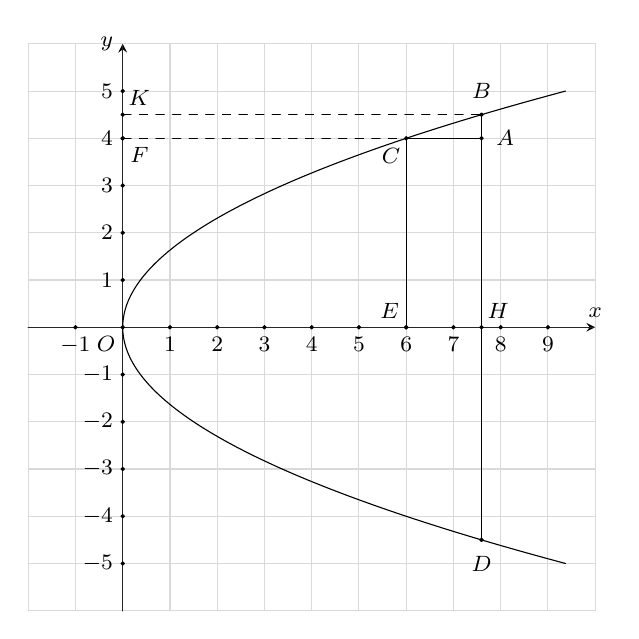
\begin{tikzpicture}[scale=0.6, font=\footnotesize, line join=round, line cap=round, >=stealth]
				\def\xB{4.5};
				\pgfmathsetmacro\yB{(3/8)*(\xB)^2};
				\path
				(0,0) coordinate (O)
				(6,0) coordinate (E)
				(6,4) coordinate (C)
				(0,4.5) coordinate (K)
				(0,4) coordinate (F)
				(\yB,\xB) coordinate (B)
				(\yB,0) coordinate (H)
				(\yB,4) coordinate (A)
				(\yB,-\xB) coordinate (D)
				;
				\draw[->] (-2,0)--(10,0) node[above]{$x$};
				\draw[->] (0,-6)--(0,6) node[left]{$y$};
				\draw[color=gray,opacity=0.3] (-2,-6) grid (10,6);
				\clip (-2,-6) rectangle (10,6);
				\draw[rotate=-90,smooth, samples=200, domain=-5:5] plot (\x,{(3/8)*(\x)^2});
				\draw (E)--(C)--(A) (B)--(D);
				\draw[dashed] (K)--(B) (F)--(C);
				\foreach \i/\g in {A/0,B/90,C/-130,D/-90,E/135,F/-45,H/45,K/45,O/-135} \draw[fill=black] (\i) circle(1pt)++(\g:0.5) node{$\i$};
				\foreach \j in {-1,1,2,3,4,5,6,7,8,9} \draw[fill=black](\j,0) circle(1pt) node[below]{$\j$};
				\foreach \k in {-5,-4,-3,-2,-1,1,2,3,4,5} \draw[fill=black](0,\k) circle(1pt) node[left]{$\k$};
			\end{tikzpicture}
		}
	}
\end{vd}

\begin{bt} 
	Một cái cầu có dây cáp treo hình parabol, cầu dài $100$ m và được nâng đỡ bởi những thanh thẳng đứng treo từ cáp xuống, thanh dài nhất là $30$ m, thanh ngắn nhất là $6$ m (hình bên dưới). Tính chiều dài của thanh cách điểm giữa cầu $18$ m.
	\begin{center}
		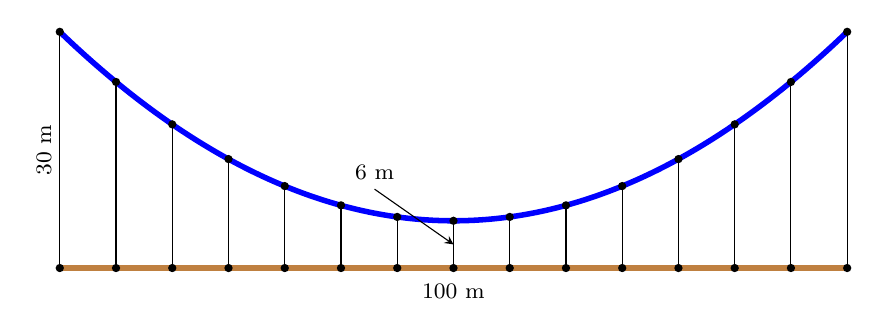
\begin{tikzpicture}[scale=1, font=\footnotesize, line join=round, line cap=round, >=stealth]
			\tikzset{thanh-cau/.pic={
					\pgfmathsetmacro\k{5/7};
					\draw[line width=2pt,blue,smooth,samples=100, domain=-5:5] plot (\x,{(12/125)*(\x)^2+0.6});
					\foreach \i in {-7,-6,...,7} \draw ({(\k)*(\i)},0)--({(\k)*(\i)},{(12/125)*((\k)*(\i))^2+0.6});
					\draw[line width=2pt,brown] (-5,0)--(5,0);
					\foreach \i in {-7,-6,...,7} \fill[black] ({(\k)*(\i)},0) circle (1.5pt);
					\foreach \i in {-7,-6,...,7} \fill[black] ({(\k)*(\i)},{(12/125)*((\k)*(\i))^2+0.6}) circle (1.5pt);
			}}
			\path (0,0)pic{thanh-cau};
			\draw (-5.2,1.5) node[rotate=90]{$30$ m};
			\draw (0,-0.3) node{$100$ m};
			\draw[<-] (0,0.3)--(-1,1) node[above]{$6$ m};
		\end{tikzpicture}
	\end{center}
	\loigiai{
		\immini{
			Ta chọn hệ tọa độ sao cho parabol $(P)$ có phương trình $y^2=2px$ \quad $(1)$.\\
			Thay tọa độ điểm $M(24;50)$ vào phương trình $(1)$, ta được $$50^2=2p\cdot 24\Leftrightarrow p=\dfrac{625}{12}.$$
			Khi đó $(P)\colon y^2=\dfrac{625}{6}x$.\\
			Thay tọa độ điểm $N(x_N;18)$ vào phương trình $(P)$, ta được $$18^2=\dfrac{625}{6}\cdot x_N\Rightarrow x_N=\dfrac{1944}{625}=3{,}1104.$$
			Vậy chiều dài của thanh cách điểm giữa cầu $18$ m là $$3{,}1104+6=9{,}1104\text{ (m).}$$
		}{
			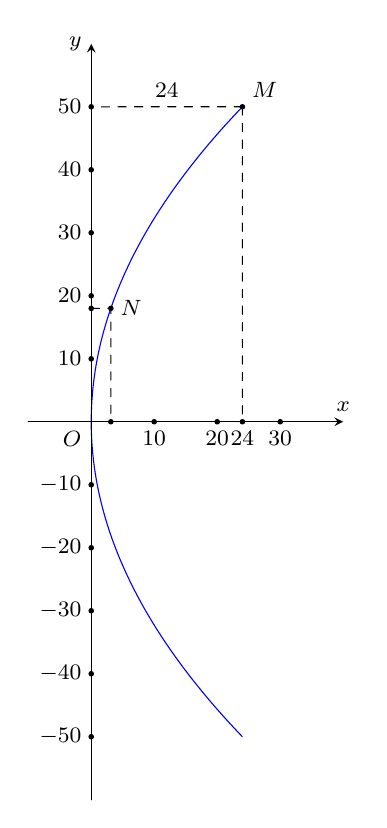
\begin{tikzpicture}[scale=0.8, font=\footnotesize, line join=round, line cap=round, >=stealth]	
				\draw[rotate=-90,blue,smooth,samples=100, domain=-5:5] plot (\x,{(12/125)*(\x)^2});
				\draw[->] (-1,0)--(4,0) node[above]{$x$};
				\draw[->] (0,-6)--(0,6) node[left]{$y$};
				\draw[fill=black] (0,0) node[below left]{$O$};
				\draw [fill=black](2.4,5) coordinate(M) circle(1pt) node[above right]{$M$};
				\draw [fill=black](0.31104,1.8) coordinate(N) circle(1pt) node[right]{$N$};
				\foreach \i/\m in {1/10,2/20,3/30} \draw[fill=black] (\i,0) circle(1pt) node[below]{$\m$};
				\foreach \j/\n in {-5/-50,-4/-40,-3/-30,-2/-20,-1/-10,1/10,2/20,3/30,4/40,5/50} \draw[fill=black] (0,\j) circle(1pt) node[left]{$\n$};
				\draw[dashed] (M)--(0,5) node[above,pos=0.5]{$24$};
				\draw[dashed] (M)--(2.4,0) coordinate(M_1);
				\draw[dashed] (0,1.8) coordinate(N_2)--(N)--(0.31104,0) coordinate(N_1);
				\draw[fill=black] (M_1) circle(1pt)  node[below]{$24$};
				\draw[fill=black] (N_1) circle(1pt);
				\draw[fill=black] (N_2) circle(1pt);
			\end{tikzpicture}
		}
	}
\end{bt}

\begin{bt} 
	\immini{
		Cổng chào của một thành phố dạng hình parabol có chiều cao $h=25\mathrm{m}$ và khoảng cách giữa hai chân cổng là $d=120\mathrm{m}$. Hãy viết phương trình parabol của cổng chào.
	}{
		\begin{tikzpicture}[font=\footnotesize, line join=round, line cap=round, >=stealth,scale=0.3]
			\tikzset{Cong-chao/.pic={
					\def\cao{5}
					\def\rong{6}
					\fill[green!60](-10,0)rectangle(15,10);
					\fill[gray!40,draw=gray!60](-10,0)rectangle(15,-2);
					\fill[cyan!20](-10,2.45)rectangle(15,10);
					\fill[red!30!brown](-\rong-1,0)--++(26:5.65)--++(0:3.75)--(\rong+1,0)--cycle;
					%\fill[cyan](-10,2.25)rectangle(5,15);
					\fill[pattern color=white,pattern=bricks,orange,samples=100,domain=-\rong:\rong]plot(\x,{(-\cao/36)*(\x-\rong)*(\x+\rong)})[samples=100,domain=\rong+1:-\rong-1]plot(\x,{(-0.85*\cao/36)*(\x-\rong-1)*(\x+\rong+1)});
					\fill[pattern color=white,pattern=bricks,draw=brown,samples=100,domain=-\rong:\rong]plot(\x,{(-\cao/36)*(\x-\rong)*(\x+\rong)})[samples=100,domain=\rong+1:-\rong-1]plot(\x,{(-0.85*\cao/36)*(\x-\rong-1)*(\x+\rong+1)});
					\fill[gray,draw=brown,samples=100,domain=-\rong:\rong]plot(\x,{(-\cao/36)*(\x-\rong)*(\x+\rong)})[samples=100,domain=\rong-1:-\rong+1]plot(\x,{1.35*(-\cao/36)*(\x-\rong+1)*(\x+\rong-1)});
					\fill[gray!50,draw=gray!50](-\rong,0)--++(30:5)--++(0:3)--(\rong,0);
					\fill[white,yscale=0.3,xscale=0.5](-1,0)--(-0.5,3)--(0.5,3)--(1,0)--cycle;
					\fill[shift={(0,1.5)},white,yscale=0.5,xscale=0.5,scale=0.5](-1,0)--(-0.5,3)--(0.5,3)--(1,0)--cycle;
			}}
			\path(0,0)pic[scale=0.5]{Cong-chao};
			
		\end{tikzpicture}
	}
	\loigiai{
		\immini{
			Ta chọn hệ tọa độ như hình bên.\\
			Gọi parabol có phương trình của parabol có dạng $y^2=2px$.\\
			Ta có $M(25;60)$ là tọa độ một điểm tại chân cổng chào.\\
			Thay tọa độ điểm $M$ vào phương trình $(P)$ ta có $60^2=2p \cdot 25 \Rightarrow p=\dfrac{60^2}{50}=72$.\\
			Vậy phương trình của $(P)$ là $y^2=144x$.
		}{
			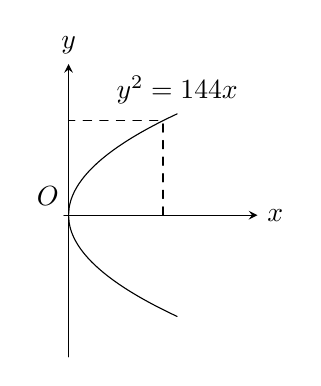
\begin{tikzpicture}[domain=0:2.3,line join = round, line cap = round,>=stealth,scale=0.6]
				\draw[->] (-0.1,0) -- (4,0) node[right] {$x$};
				\draw[->] (0,-3) -- (0,3.2) node[above] {$y$};
				\draw(0,0)node[above left]{$O$};
				\draw[smooth, samples=150] plot (\x,{-(2*(\x))^(0.5)});
				\draw[smooth, samples=150] plot (\x,{(2*(\x))^(0.5)}) node[above]{$y^2=144x$};
				\draw[dashed] (2,0)--(2,2)--(0,2);
			\end{tikzpicture}  
		}
	}
\end{bt}

\begin{bt}
	Gương phản chiếu của của một đèn qua có mặt cắt là một parabol $(P)$ với bóng đèn đặt tại tiêu điểm $F$. Chiều rộng giữa hai mép gương là $50$ cm. Chiều sâu của gương là $40$ cm. Viết phương trình chính tắc của parabol.
	
	\loigiai{
		\begin{center}
			\begin{tikzpicture}[>=stealth,line join=round,line cap=round,font=\footnotesize,scale=1,rotate=-90]
				\draw[->] (2,0)--(-2,0)node[right]{$x$};
				\draw[->]	(0,-.5)--(0,4)node[below]{$y$};
				\draw[domain=-1.5:1.5,samples=100] plot (\x,{(\x)^2}) ;                                  
				\fill (0,.5)circle(0.03) node[below]{$F$}
				
				
				
				;
				\draw (0,0)node[below left]{$O$};
				\draw[dashed] (-1.5, 2.25)node[above]{$M$}--(1.5, 2.25)node[below]{$N$};
				\fill (0,2.25)node[below right]{$H$};
			\end{tikzpicture}
		\end{center}
		Mô hình bài toán có dạng như hình vẽ.\\
		Theo bài ra ta có $MN=50$, $OH=40$, suy ra $M(40;25)$.\\
		Giả sử parabol có phương trình chính tắc dạng $y^2=2px$.\\
		Do $H$ thuộc parabol nên $25^2=2p\cdot 40\Rightarrow p\approx 7{,}8$.\\
		Vậy phương trình chính tắc của parabol là $y^2=15{,}6x$.
	}
\end{bt}
\newpage
%\begin{dang}{Bài toán thực tế}
%\end{dang}
%\begin{vd}
%	Đường thẳng $\Delta$ ở hình bên dưới biểu thị tổng chi phí lắp đặt và tiền cước sử dụng dịch vụ Internet (đơn vị: trăm nghìn đồng) theo thời gian của một gia đình (đơn vị: tháng).\\
%	\begin{enumerate}
%		\item Viết phương trình của đường thẳng $\Delta$.
%		\item Cho biết giao điểm của đường thẳng $\Delta$ với trục tung trong tình huống này có ý nghĩa gì.
%		\item Tính tổng chi phí lắp đặt và sử dụng Internet trong $12$ tháng đầu tiên.
%	\end{enumerate}
%	\begin{center}
%		\begin{tikzpicture}[scale=0.8, font=\footnotesize, line join=round, line cap=round, >=stealth]
%			\draw[->,line width = 1pt] (-1,0)--(0,0) node[below left]{$O$}--(6.5,0) node[below]{$x$};
%			\draw[->,line width =1 pt] (0,-1)--(0,5) node[right]{$y$};
%			\draw [thick,domain=0:6,samples=100] 
%			plot (\x,{(3/5)*(\x)+1/2}) node [above left] {$\Delta$};
%			\draw (0,0.5) node [left] {$5$} circle (1pt);
%			\draw (0,1) node [left] {$10$} circle (1pt);		
%			\draw (0,2) node [left] {$20$} circle (1pt);
%			\draw (0.5,0) node [below] {$1$} circle (1pt);
%			\draw (2.5,0) node [below] {$5$} circle (1pt);
%			\draw (6,0) node [below] {$12$} circle (1pt);
%			\draw [dashed] (2.5,0)--(2.5,2)--(0,2);
%		\end{tikzpicture}	
%	\end{center}
%	\loigiai{
%		\begin{enumerate}
%			\item Đường thẳng $\Delta$ đi qua hai điểm lần lượt có tọa độ $(0;\,5)$ và $(5;\,20)$ nên $\Delta$ có phương trình là
%			$$\dfrac{x-0}{5-0}=\dfrac{y-5}{20-5}\Leftrightarrow\dfrac{x}{5}=\dfrac{y-5}{15}\Leftrightarrow\dfrac{x}{1}=\dfrac{y-5}{3}\Leftrightarrow3x-y+5=0\Leftrightarrow y=3x+5.$$
%			\item Giao điểm của đường thẳng $\Delta$ với trục $Oy$ ứng với $x=0$. Thời điểm $x=0$ cho biết mức phí ban đầu lắp đặt để sử dụng Internet. Khi $x=0$ thì $y=5$, vì vậy chi phí lắp đặt ban đầu là $500000$ đồng.
%			\item $12$ tháng đầu tiên ứng với $x=12$. Do đó $y=3\cdot12+5=41$.\\
%			Vậy tổng chi phí lắp đặt và sử dụng Internet trong $12$ tháng đầu tiên là $4100000$ đồng.
%		\end{enumerate}
%		
%	}
%\end{vd}
%\begin{vd}
%	Để tham gia một phòng tập thể dục, người tập phải trả một khoản phí tham gia ban đầu và phí sử dụng phòng tập. Đường thẳng $\Delta$ ở hình bên dưới biểu thị tổng chi phí (đơn vị: triệu đồng) tham gia một phòng tập thể dục theo thời gian tập của một người (đơn vị: tháng).\\
%	\begin{enumerate}
%		\item Viết phương trình của đường thẳng $\Delta$.
%		\item Cho biết giao điểm của đường thẳng $\Delta$ với trục tung trong tình huống này có ý nghĩa gì.
%		\item Tính tổng chi phí mà người đó phải trả khi tham gia phòng tập thể dục với thời gian $12$ tháng.
%	\end{enumerate}
%	\begin{center}
%		\begin{tikzpicture}[scale=0.8, font=\footnotesize, line join=round, line cap=round, >=stealth]
%			\draw[->,line width = 1pt] (-1,0)--(0,0) node[below left]{$O$}--(8,0) node[below]{$x$};
%			\draw[->,line width =1 pt] (0,-1)--(0,8) node[right]{$y$};
%			\draw [thick,domain=0:6,samples=100] 
%			plot (\x,{(\x)+3/2}) node [above left] {$\Delta$};
%			\draw (0,1) node [left] {$1$} circle (1pt);
%			\draw (0,1.5) node [left] {$1{,}5$} circle (1pt);		
%			\draw (0,5) node [left] {$5$} circle (1pt);
%			\draw (0.5,0) node [below] {$1$} circle (1pt);
%			\draw (3.5,0) node [below] {$7$} circle (1pt);
%			\draw (6,0) node [below] {$12$} circle (1pt);
%			\draw [dashed] (3.5,0)--(3.5,5)--(0,5);
%		\end{tikzpicture}	
%	\end{center}
%	\loigiai{
%		\begin{enumerate}
%			\item Đường thẳng $\Delta$ đi qua hai điểm lần lượt có tọa độ $(0;\,1{,}5)$ và $(7;\,5)$ nên $\Delta$ có phương trình là
%			$$\dfrac{x-0}{7-0}=\dfrac{y-1{,}5}{5-1{,}5}\Leftrightarrow\dfrac{x}{7}=\dfrac{y-1{,}5}{3{,}5}\Leftrightarrow\dfrac{x}{2}=\dfrac{y-1{,}5}{1}\Leftrightarrow y=\dfrac{x}{2}+1{,}5.$$
%			\item Giao điểm của đường thẳng $\Delta$ với trục $Oy$ ứng với $x=0$. Thời điểm $x=0$ cho biết mức phí tham gia ban đầu và phí sử dụng phòng tập. Khi $x=0$ thì $y=1{,}5$, vì vậy chi phí tham gia ban đầu và phí sử dụng phòng tập là $1500000$ đồng.
%			\item $12$ tháng đầu tiên ứng với $x=12$. Do đó $y=\dfrac{12}{2}+1{,}5=7{,}5$.\\
%			Vậy tổng chi phí mà người đó phải trả khi tham gia phòng tập thể dục với thời gian $12$ tháng đầu tiên là $7500000$ đồng.
%		\end{enumerate}
%		
%	}
%\end{vd}
%
%
%\subsection{Bài tập tự luận}
%\begin{bt}%[0H3B1-2]
%	Trong mặt phẳng $Oxy$, cho $\overrightarrow{n}=(2;1)$, $\overrightarrow{v}=(3;2)$, $A(1;3)$, $B(-2;1)$.
%	\begin{enumerate}
%		\item Lập phương trình tổng quát của đường thẳng $\Delta_1$ đi qua $A$ và có véc-tơ pháp tuyến $\overrightarrow{n}$.
%		\item Lập phương trình tham số của đường thẳng $\Delta_2$ đi qua $B$ và có véc-tơ chỉ phương $\overrightarrow{v}$.
%		\item Lập phương trình tham số của đường thẳng $AB$.
%	\end{enumerate}
%	\loigiai{
%		\begin{enumerate}
%			\item Phương trình tổng quát của $\Delta_1\colon 2\cdot(x-1)+1\cdot(y-3)=0$ hay $\Delta_1\colon 2x+y-5=0$.
%			\item Phương trình tham số của $\Delta_2\colon \heva{&x=-2+3t\\&y=1+2t}\quad (t\in\mathbb{R})$.
%			\item Ta có $\overrightarrow{AB}=(-3;-2)$ là một véc-tơ chỉ phương của đường thẳng $AB$.\\
%			Phương trình tham số của đường thẳng $AB\colon \heva{&x=1-3s\\&y=3-2s} \quad (s\in\mathbb{R})$.
%		\end{enumerate}	
%	}
%\end{bt}
%
%\begin{bt}%[0H3B1-2]
%	Trong mặt phẳng $Oxy$, lập phương trình tổng quát các trục tọa độ.
%	\loigiai{
%		\begin{enumerate}
%			\item Trục $Ox$ có véc-tơ pháp tuyến là $\overrightarrow{j}=(0;1)$ nên phương trình tổng quát của \linebreak $Ox\colon 0\cdot(x-1)+1\cdot(y-0)=0$ hay $Ox\colon y=0$.
%			\item Tương tự, phương trình tổng quát của $Oy\colon x=0$.
%		\end{enumerate}
%	}
%\end{bt}
%
%\begin{bt}%[0H3B1-2]
%	Trong mặt phẳng $Oxy$, cho hai đường thẳng $\Delta_1\colon \heva{&x=1+2t\\&y=3+5y}$ và $\Delta_2\colon 2x+3y-5=0$.
%	\begin{enumerate}
%		\item Lập phương trình tổng quát của $\Delta_1$.
%		\item Lập phương trình tham số của $\Delta_2$.
%	\end{enumerate}
%	\loigiai{
%		\begin{enumerate}
%			\item Ta có $\Delta_1\colon \heva{&x=1+2t\\&y=3+5y} \Rightarrow 5x-2y+1=0$.\\
%			Vậy phương trình tổng quát của $\Delta_1\colon 5x-2y+1=0$.
%			\item Chọn $x=1+3s$ suy ra $y=1-2s$.\\
%			Vậy phương trình tham số của $\Delta_2\colon \heva{&x=1+3s\\&y=1-2s} \quad (s\in\mathbb{R})$.
%		\end{enumerate}
%	}
%\end{bt}
%
%\begin{bt}%[0H3B1-2]
%	Trong mặt phẳng $Oxy$, cho tam giác $ABC$ có $A(1;2)$, $B(3;0)$ và $C(-2;-1)$.
%	\begin{enumerate}
%		\item Lập phương trình đường cao kẻ từ $A$.
%		\item Lập phương trình đường trung tuyến kẻ từ $B$.
%	\end{enumerate}
%	\loigiai{
%		\begin{enumerate}
%			\item Gọi $AH$ là đường cao kẻ từ $A$.\\
%			Ta có $AH$ nhận $\overrightarrow{n}=-\overrightarrow{BC}=(5;1)$ là véc-tơ pháp tuyến.\\
%			Phương trình tổng quát của đường cao $AH\colon 5\cdot(x-1)+1\cdot(y-2)=0$ hay $AH\colon 5x+y-7=0$.
%			\item Ta có $M\left(-\dfrac{1}{2};\dfrac{1}{2}\right)$ là trung điểm của $AC$.\\
%			Đường trung tuyến $BM$ nhận $\overrightarrow{u}=-2\overrightarrow{BM}=(7;-1)$ là véc-tơ chỉ phương.\\
%			Phương trình tham số của $BM\colon \heva{&x=3+7t\\&y=-t} \quad (t\in\mathbb{R})$.
%		\end{enumerate}
%	}
%\end{bt}
%
%\begin{bt}%[0H3B1-2]
%	Trong mặt phẳng $Oxy$, chứng minh rằng đường thẳng đi qua hai điểm $A(a;0)$, $B(0;b)$ với $ab\ne 0$ có phương trình là $\dfrac{x}{a}+\dfrac{y}{b}=1$. (phương trình đoạn chắn của đường thẳng)
%	\loigiai{
%		Gọi $\Delta\colon \dfrac{x}{a}+\dfrac{y}{b}=1$.\\
%		Ta có $\heva{&\dfrac{a}{a}+\dfrac{0}{b}=1\quad\text{(luôn đúng)}\\&\dfrac{0}{a}+\dfrac{b}{b}=1\quad\text{(luôn đúng)}} \Rightarrow \heva{&A\in\Delta\\&B\in\Delta.}$\\
%		Vậy phương trình của $AB\colon \dfrac{x}{a}+\dfrac{y}{b}=1$.
%	}
%\end{bt}
%
%\begin{bt}%[0H3B1-7]
%	Theo Google Maps, sân bay Nội Bài có vĩ độ $21{,}2^\circ$ Bắc, kinh độ $105{,}8^\circ$ Đông, sân bay Đà Nẵng có vĩ độ $16{,}1^\circ$ Bắc, kinh độ $108{,}2^\circ$ Đông. Một máy bay, bay từ sân bay Nội Bài đến sân bay Đà Nẵng. Tại thời điểm $t$ giờ, tính từ lúc xuất phát, máy bay ở vị trí có vĩ độ $x^\circ$ Bắc, kinh độ $y^\circ$ Đông được tính theo công thức $\heva{&x=21{,}2-\dfrac{153}{40}t\\&y=105{,}8+\dfrac{9}{5}t.}$
%	\begin{enumerate}
%		\item Hỏi chuyến bay từ Nội Bài đến Đà Nẵng mất mấy giờ?
%		\item Tại thời điểm $1$ giờ kể từ lúc cất cánh, máy bay đã bay qua vĩ tuyến $17$ ($17^\circ$ Bắc) chưa?
%	\end{enumerate}
%	\loigiai{
%		\begin{enumerate}
%			\item Xét $x=16{,}1 \Leftrightarrow 21{,}2-\dfrac{153}{40}t=16{,}1 \Leftrightarrow t=\dfrac{4}{3}$ giờ.
%			\item Tại thời điểm $1$ giờ, máy bay ở vĩ độ $x=21{,}2-\dfrac{153}{40}\cdot 1=17{,}37$.\\
%			Vậy máy bay chưa bay qua vĩ tuyến $17$ ($17^\circ$ Bắc).
%		\end{enumerate}
%	}
%\end{bt}
%\subsection{Bài tập trắc nghiệm}
%\Opensolutionfile{ans}[ans]
%% Câu 1
%\begin{ex}%[0H3Y1-2]
%	Đường thẳng đi qua $A\left(-1; 2\right)$, nhận $\overrightarrow{n}=(2;-4)$ làm véctơ pháp tuyến có phương trình là
%	\choice
%	{$x+2y+4=0$}
%	{\True $x-2y+5=0$}
%	{$x-2y-4=0$}
%	{$x+y+4=0$}
%	\loigiai{
%		Đường thẳng đi qua $A\left(-1; 2\right)$, nhận $\overrightarrow{n}=(2;-4)$ làm véctơ pháp tuyến có phương trình là
%		\[2\left(x+1\right)-4\left(y-2\right)=0\Leftrightarrow x-2y+5=0.\]
%	}
%\end{ex}
%% Câu 2
%\begin{ex}%[0H3Y1-2]
%	Đường thẳng đi qua điểm $M\left(1;2\right)$ và vuông góc với vec-tơ $\overrightarrow{n}=\left(2;3\right)$ có phương trình chính tắc là
%	\choice
%	{$\dfrac{x-1}{2}=\dfrac{y-2}{3}$}
%	{\True $\dfrac{x-1}{3}=\dfrac{y-2}{-2}$}
%	{$\dfrac{x+1}{2}=\dfrac{y+2}{3}$}
%	{$\dfrac{x+1}{-3}=\dfrac{y+2}{2}$}
%	\loigiai{
%		Ta có vec-tơ pháp tuyến của đường thẳng là $\overrightarrow{n}=\left(2;3\right)$, do đó vec-tơ chỉ phương của đường thẳng là $\overrightarrow{u}=\left(3;-2\right)$.\\
%		Phương trình chính tắc của đường thẳng đi qua $M\left(1;2\right)$ và có vec-tơ chỉ phương $\overrightarrow{u}=\left(3;-2\right)$ là $\dfrac{x-1}{3}=\dfrac{y-2}{-2}$.}
%\end{ex}
%% Câu 3
%\begin{ex}%[0H3B1-2]
%	Cho tam giác $ABC$ có $A(2;0), B(0;3), C(-3;1)$. Đường thẳng qua $B$ và song song với $AC$ có phương trình là
%	\choice
%	{$x-5y+15=0$}
%	{$5x-y+3=0$}
%	{$5x+y-3=0$}
%	{\True $x+5y-15=0$}
%	\loigiai{
%		Ta có $\overrightarrow{AC}=(-5;1)$, vậy phương trình đường thẳng cần tìm là $\dfrac{x-0}{-5}=\dfrac{y-3}{1}\Leftrightarrow x+5y-15=0$.}
%\end{ex}
%% Câu 4
%\begin{ex}%[0H3B1-2]
%	Viết phương trình đường thẳng qua giao điểm của hai đường thẳng $2x-y+5=0$ và $3x+2y-3=0$ và đi qua điểm $A(-3;-2)$
%	\choice
%	{\True $5x-2y+11=0$}
%	{$2x-5y+11=0$}
%	{$5x+2y+11=0$}
%	{$x-y-3=0$}
%	\loigiai{
%		Gọi $B$ là tọa độ giao điểm của 2 đường thẳng.\\
%		Tọa độ $B$ thỏa mãn hệ \[\heva{
%			& 2x-y+5=0 \\ 
%			& 3x+2y-3=0 \\}\Leftrightarrow \heva{
%			& 2x-y=-5 \\ 
%			& 3x+2y=3 \\}\Leftrightarrow \heva{
%			& x=-1 \\ 
%			& y=3 \\}\Rightarrow B\left(-1;3\right).\]
%		Ta có $\overrightarrow{AB}=\left(2;5\right)$, khi đó $\overrightarrow{n}_{AB}=\left(5;-2\right)$.\\
%		Phương trình đường thẳng là $AB\colon 5\left(x+3\right)-2\left(y+2\right)=0\Leftrightarrow 5x-2y+11=0$.}
%\end{ex}
%% Câu 5
%\begin{ex}%[0H3B1-2]
%	Cho hai điểm $A(4;-1);B(1;-4)$. Viết phương trình tổng quát đường trung trực của đoạn thẳng $AB$.
%	\choice
%	{$x-y=0$}
%	{$x-y=1$}
%	{$x+y=1$}
%	{\True $x+y=0$}
%	\loigiai{
%		$\overrightarrow{AB}=(-3;-3)=-3(1;1)$. Gọi $M$ là trung điểm của $AB$ thì $M\left(\dfrac{5}{2};-\dfrac{5}{2}\right)$.\\
%		Đường trung trực của đoạn thẳng $AB$ đi qua $M\left(\dfrac{5}{2};-\dfrac{5}{2}\right)$ và nhận $\overrightarrow{n}=(1;1)$ làm một vec-tơ pháp tuyến nên có phương trình tổng quát  \[\left(x-\dfrac{5}{2}\right)+\left(y+\dfrac{5}{2}\right)=0\Leftrightarrow x+y=0.\]}
%\end{ex}
%% Câu 6
%\begin{ex}%[0H3Y1-2]
%	Cho đường thẳng $\Delta\colon y=-\dfrac{3}{2}x+1$. Vec-tơ nào sau đây không là vec-tơ chỉ phương của $\Delta $?
%	\choice
%	{\True $\left(-3;2\right)$}
%	{$\left(2;3\right)$}
%	{$\left(1;-\dfrac{3}{2}\right)$}
%	{$\left(-2;3\right)$}
%	\loigiai{
%		Đường thẳng $\Delta\colon y=-\dfrac{3}{2}x+1$ có hệ số góc $k=-\dfrac{3}{2}=\dfrac{u_2}{u_1}$, với $\overrightarrow{u}=\left(u_1;u_2\right)$ là VTCP của $\Delta $.\\
%		Loại trừ các VTCP của $\Delta $ khi chọn $u_1=\left\{1;2;-2\right\}$.\\
%		Vậy vec-tơ không là VTCP cần tìm là $\left(-3;2\right)$.}
%\end{ex}
%% Câu 7
%\begin{ex}%[0H3B1-2]
%	Viết phương trình tham số của đường thẳng đi qua điểm $O\left(0;0\right)$ và song song với đường thẳng $\Delta \colon 3x-4y+1$.
%	\choice
%	{$\heva{
%			& x=-3t \\ 
%			& y=4t \\}$}
%	{$\heva{
%			& x=3t \\ 
%			& y=-4t \\}$}
%	{\True $\heva{
%			& x=4t \\ 
%			& y=3t \\}$}
%	{$\heva{
%			& x=4t \\ 
%			& y=1+3t \\}$}
%	\loigiai{
%		Thay tọa độ điểm $O$ vào phương trình đường thẳng $\Delta $ thấy không thỏa mãn.\\
%		Do hai đường thẳng song song nên đường thẳng cần tìm nhận $\overrightarrow{u}\left(4;3\right)$ làm vec-tơ chỉ phương.\\
%		Phương trình tham số của đường thẳng cần tìm $\heva{
%			& x=4t \\ 
%			& y=3t. \\}$
%	}
%\end{ex}
%% Câu 8
%\begin{ex}%[0H3B1-2]
%	Cho tam giác $ABC$ có tọa độ các đỉnh là $A\left(1;2\right)$, $B\left(3;1\right)$, và $C\left(5;4\right)$. Phương trình nào sau đây là phương trình đường cao của tam giác vẽ từ $A$?
%	\choice
%	{$5x-6y+7=0$}
%	{$3x-2y+5=0$}
%	{\True $2x+3y-8=0$}
%	{$3x-2y-5=0$}
%	\loigiai{
%		Đường cao vẽ từ $A$ đi qua điểm $A\left(1;2\right)$ và nhận $\overrightarrow{BC}=\left(2;3\right)$ làm vec tơ pháp tuyến có phương trình $2x+3y-8=0$.}
%\end{ex}
%% Câu 9
%\begin{ex}%[0H3Y1-2]
%	Cho đường thẳng $\Delta \colon \heva{
%		& x=15 \\ 
%		& y=6+7t \\}$. Viết phương trình tổng quát của $\Delta $.
%	\choice
%	{$x+15=0$}
%	{$6x-15y=0$}
%	{\True $x-15=0$}
%	{$x-y-9=0$}
%	\loigiai{
%		Đường thẳng có vtcp $\overrightarrow{u}=\left(0;7\right)$ nên có vtpt $\overrightarrow{n}=\left(1;0\right)$.\\
%		Đường thẳng $\Delta $ đi qua điểm $\left(15;6\right)$ nên có phương trình tổng quát là $x-15=0$.}
%\end{ex}
\Closesolutionfile{ans}